\documentclass[a4paper]{report}
% Some basic packages
\usepackage[utf8]{inputenc}
\usepackage[T1]{fontenc}
\usepackage{textcomp}
\usepackage[english]{babel}
\usepackage{url}
\usepackage{graphicx}
\usepackage{float}
\usepackage{booktabs}
\usepackage{enumitem}

\pdfminorversion=7

% Don't indent paragraphs, leave some space between them
\usepackage{parskip}

% Hide page number when page is empty
\usepackage{emptypage}
\usepackage{subcaption}
\usepackage{multicol}
\usepackage{xcolor}

% Other font I sometimes use.
% \usepackage{cmbright}

% Math stuff
\usepackage{amsmath, amsfonts, mathtools, amsthm, amssymb}
% Fancy script capitals
\usepackage{mathrsfs}
\usepackage{cancel}
% Bold math
\usepackage{bm}
% Some shortcuts
\newcommand\N{\ensuremath{\mathbb{N}}}
\newcommand\R{\ensuremath{\mathbb{R}}}
\newcommand\Z{\ensuremath{\mathbb{Z}}}
\renewcommand\O{\ensuremath{\emptyset}}
\newcommand\Q{\ensuremath{\mathbb{Q}}}
\newcommand\C{\ensuremath{\mathbb{C}}}
\renewcommand\L{\ensuremath{\mathcal{L}}}

% Package for Petri Net drawing
\usepackage[version=0.96]{pgf}
\usepackage{tikz}
\usetikzlibrary{arrows,shapes,automata,petri}
\usepackage{tikzit}
\input{petri_nets_style.tikzstyles}

% Easily typeset systems of equations (French package)
\usepackage{systeme}

% Put x \to \infty below \lim
\let\svlim\lim\def\lim{\svlim\limits}

%Make implies and impliedby shorter
\let\implies\Rightarrow
\let\impliedby\Leftarrow
\let\iff\Leftrightarrow
\let\epsilon\varepsilon

% Add \contra symbol to denote contradiction
\usepackage{stmaryrd} % for \lightning
\newcommand\contra{\scalebox{1.5}{$\lightning$}}

% \let\phi\varphi

% Command for short corrections
% Usage: 1+1=\correct{3}{2}

\definecolor{correct}{HTML}{009900}
\newcommand\correct[2]{\ensuremath{\:}{\color{red}{#1}}\ensuremath{\to }{\color{correct}{#2}}\ensuremath{\:}}
\newcommand\green[1]{{\color{correct}{#1}}}

% horizontal rule
\newcommand\hr{
    \noindent\rule[0.5ex]{\linewidth}{0.5pt}
}

% hide parts
\newcommand\hide[1]{}

% si unitx
\usepackage{siunitx}
\sisetup{locale = FR}

% Environments
\makeatother
% For box around Definition, Theorem, \ldots
\usepackage{mdframed}
\mdfsetup{skipabove=1em,skipbelow=0em}
\theoremstyle{definition}
\newmdtheoremenv[nobreak=true]{definitie}{Definitie}
\newmdtheoremenv[nobreak=true]{eigenschap}{Eigenschap}
\newmdtheoremenv[nobreak=true]{gevolg}{Gevolg}
\newmdtheoremenv[nobreak=true]{lemma}{Lemma}
\newmdtheoremenv[nobreak=true]{propositie}{Propositie}
\newmdtheoremenv[nobreak=true]{stelling}{Stelling}
\newmdtheoremenv[nobreak=true]{wet}{Wet}
\newmdtheoremenv[nobreak=true]{postulaat}{Postulaat}
\newmdtheoremenv{conclusie}{Conclusie}
\newmdtheoremenv{toemaatje}{Toemaatje}
\newmdtheoremenv{vermoeden}{Vermoeden}
\newtheorem*{herhaling}{Herhaling}
\newtheorem*{intermezzo}{Intermezzo}
\newtheorem*{notatie}{Notatie}
\newtheorem*{observatie}{Observatie}
\newtheorem*{exe}{Exercise}
\newtheorem*{opmerking}{Opmerking}
\newtheorem*{praktisch}{Praktisch}
\newtheorem*{probleem}{Probleem}
\newtheorem*{terminologie}{Terminologie}
\newtheorem*{toepassing}{Toepassing}
\newtheorem*{uovt}{UOVT}
\newtheorem*{vb}{Voorbeeld}
\newtheorem*{vraag}{Vraag}

\newmdtheoremenv[nobreak=true]{definition}{Definition}
\newtheorem*{eg}{Example}
\newtheorem*{notation}{Notation}
\newtheorem*{previouslyseen}{As previously seen}
\newtheorem*{remark}{Remark}
\newtheorem*{note}{Note}
\newtheorem*{problem}{Problem}
\newtheorem*{observe}{Observe}
\newtheorem*{property}{Property}
\newtheorem*{intuition}{Intuition}
\newmdtheoremenv[nobreak=true]{prop}{Proposition}
\newmdtheoremenv[nobreak=true]{theorem}{Theorem}
\newmdtheoremenv[nobreak=true]{corollary}{Corollary}

% End example and intermezzo environments with a small diamond (just like proof
% environments end with a small square)
\usepackage{etoolbox}
\AtEndEnvironment{vb}{\null\hfill$\diamond$}%
\AtEndEnvironment{intermezzo}{\null\hfill$\diamond$}%
% \AtEndEnvironment{opmerking}{\null\hfill$\diamond$}%

% Fix some spacing
% http://tex.stackexchange.com/questions/22119/how-can-i-change-the-spacing-before-theorems-with-amsthm
\makeatletter
\def\thm@space@setup{%
  \thm@preskip=\parskip \thm@postskip=0pt
}


% Exercise 
% Usage:
% \exercise{5}
% \subexercise{1}
% \subexercise{2}
% \subexercise{3}
% gives
% Exercise 5
%   Exercise 5.1
%   Exercise 5.2
%   Exercise 5.3
\newcommand{\exercise}[1]{%
    \def\@exercise{#1}%
    \subsection*{Exercise #1}
}

\newcommand{\subexercise}[1]{%
    \subsubsection*{Exercise \@exercise.#1}
}


% \lecture starts a new lecture (les in dutch)
%
% Usage:
% \lecture{1}{di 12 feb 2019 16:00}{Inleiding}
%
% This adds a section heading with the number / title of the lecture and a
% margin paragraph with the date.

% I use \dateparts here to hide the year (2019). This way, I can easily parse
% the date of each lecture unambiguously while still having a human-friendly
% short format printed to the pdf.

\usepackage{xifthen}
\def\testdateparts#1{\dateparts#1\relax}
\def\dateparts#1 #2 #3 #4 #5\relax{
    \marginpar{\small\textsf{\mbox{#1 #2 #3 #5}}}
}

\def\@lecture{}%
\newcommand{\lecture}[3]{
    \ifthenelse{\isempty{#3}}{%
        \def\@lecture{Lecture #1}%
    }{%
        \def\@lecture{Lecture #1: #3}%
    }%
    \subsection*{\@lecture}
    \marginpar{\small\textsf{\mbox{#2}}}
}



% These are the fancy headers
\usepackage{fancyhdr}
\pagestyle{fancy}

% LE: left even
% RO: right odd
% CE, CO: center even, center odd
% My name for when I print my lecture notes to use for an open book exam.
% \fancyhead[LE,RO]{Gilles Castel}

\fancyhead[RO,LE]{\@lecture} % Right odd,  Left even
\fancyhead[RE,LO]{}          % Right even, Left odd

\fancyfoot[RO,LE]{\thepage}  % Right odd,  Left even
\fancyfoot[RE,LO]{}          % Right even, Left odd
\fancyfoot[C]{\leftmark}     % Center

\makeatother




% Todonotes and inline notes in fancy boxes
\usepackage{todonotes}
\usepackage{tcolorbox}

% Make boxes breakable
\tcbuselibrary{breakable}

% Verbetering is correction in Dutch
% Usage: 
% \begin{verbetering}
%     Lorem ipsum dolor sit amet, consetetur sadipscing elitr, sed diam nonumy eirmod
%     tempor invidunt ut labore et dolore magna aliquyam erat, sed diam voluptua. At
%     vero eos et accusam et justo duo dolores et ea rebum. Stet clita kasd gubergren,
%     no sea takimata sanctus est Lorem ipsum dolor sit amet.
% \end{verbetering}
\newenvironment{verbetering}{\begin{tcolorbox}[
    arc=0mm,
    colback=white,
    colframe=green!60!black,
    title=Opmerking,
    fonttitle=\sffamily,
    breakable
]}{\end{tcolorbox}}

% Noot is note in Dutch. Same as 'verbetering' but color of box is different
\newenvironment{noot}[1]{\begin{tcolorbox}[
    arc=0mm,
    colback=white,
    colframe=white!60!black,
    title=#1,
    fonttitle=\sffamily,
    breakable
]}{\end{tcolorbox}}




% Figure support as explained in my blog post.
\usepackage{import}
\usepackage{xifthen}
\usepackage{pdfpages}
\usepackage{transparent}
\newcommand{\incfig}[1]{%
    \def\svgwidth{\columnwidth}
    \import{./figures/}{#1.pdf_tex}
}

% Fix some stuff
% %http://tex.stackexchange.com/questions/76273/multiple-pdfs-with-page-group-included-in-a-single-page-warning
\pdfsuppresswarningpagegroup=1


% My name
\author{Bruno M. Pacheco}


\title{Advanced Process Mining - Exam Summary}

\begin{document}

\section*{Four Competing Quality Criteria}

\begin{description}
    \item[Fitness] is the capacity of a model to allow for the behavior seen in the log.
    \item[Simplicity] is defined by the Occam's Razor, \emph{i.e.}, the least amount of complexity necessary.
    \item[Precision] is the characteristic of a model that does not allow for unseen behavior, \emph{i.e.}, that is not underfitting.
    \item[Generalization] is when a model does not overfits the data, \emph{i.e.}, it does not restricts itself to behavior to the examples seen in the log.
\end{description}

\begin{note}
    \emph{Occam's Razor} principle states that "one should no increase, beyond necessary, the number of entities required to explain anything".
\end{note}

\section*{Conformance Checking}

\subsection*{Precision}

In here, the escaping edges technique will be used.

To calculate the precision of a model and a log, an automaton is built upon the alignments of the traces in the log and the model. Then, the automaton is enhanced with behavioral information of the model. Finally, the automaton is used to compute precision.

\begin{definition}
    Let $L$ be an event log and $M$ be a model. Let $\Lambda$ be the set of alignments of $L$ and $M$, and $\overline{\lambda}$ the projection function of an alignment over the model (\emph{i.e.}, only model moves or synchronous moves are returned). Then, we define the \emph{alignment automaton} as $A_A=\left( Q, \Sigma, \delta, \epsilon, \omega \right) $ such that:
    \begin{itemize}
	\item The set of \emph{states} $Q$ corresponds to all prefixes of the projection of the alignments, that is $Q = \overline{\overline{lambda}\left( \Lambda \right) }$ (prefix-closure of the projection of the alignments);
	    \begin{itemize}
		\item Note that, if the model has perfect fitness, we have $Q=\overline{L}$
	    \end{itemize}
	\item The set of \emph{labels} $\Sigma$ corresponds to all activities of the log;
	\item The \emph{arcs} $\delta : Q\times \Sigma \to Q$ define the concatenation between prefixes and activities;
	\item The initial state is the one corresponding to the empty sequence $\epsilon$;
	\item The function $\omega : Q\to \R$ determines the weight of each state according to its importance for the precision computation.
	    \begin{itemize}
		\item One can define $\omega$ through the frequency a state is reached by the prefixes, \emph{i.e.}, let $s \in \overline{\lambda}\left( \Lambda \right) $, $\omega(s) =  \|\left\{ \sigma_s \in L : s = head^{|s|}(\sigma_s) \\ \right\}\|$ (amount of traces that have $s$ as a prefix).
	    \end{itemize}
    \end{itemize}
\end{definition}

Then, to calculate the precision, we must compare the automaton to the possible behavior of the model.

\begin{definition}
    Let $M$ be a model, $L$ a log, and $s$ a prefix. We define the \emph{available actions} $a_v(s, M)$ as the set of available actions given the input $s$ to model $M$,  \emph{i.e.}, the set of available transitions. Furthermore, we define the set of \emph{executed actions} $e_x(s, L)$ as the set of activities that were performed in the log after $s$, that is, $e_x(s, L) = \left\{ a_s \in \mathcal{A} : s\oplus a_s \in \overline{\lambda}\left( \Lambda \right)  \right\}$.
\end{definition}

Note that, by definition, $e_x(s) \subset a_v(s) \forall s$.

\begin{definition}
    (Escaping edges) We define the \emph{escaping edges precision} through \[
    ee_p(A_A) = \frac{1}{\sum_{s \in Q} \omega(s)}\sum_{s \in Q} \omega(s) \frac{e_x(s)}{a_v(s)}
    \] 
\end{definition}

\begin{note}
    \textbf{Watch out!} Neither the starting state ($\epsilon$) nor the ending states are counted in the \emph{escaping edges} precision metric.
\end{note}

\subsection*{Fitness}

Fitness can be computed in several ways:

\begin{description}
    \item["vanilla"] \[
    \frac{TP}{TP + FN}
\] in which $TP$ is the amount of true positives (log traces that can be replayed by the model) and $FN$ is the amount of false negatives (log traces that can not be replayed by the model).
    \item[replay fitness]  \[
	    fitness(\sigma, N)=\frac{1}{2}\left( 1 - \frac{m}{c} \right) +\frac{1}{2}\left( 1-\frac{r}{p} \right) 
    \] in which, through the replay of the trace $\sigma$ on a WF-net $N$, we count the amounts of:
    \begin{description}
        \item[$p$] produced tokens;
	\item[$c$] consumed tokens;
	\item[$m$] missing tokens; and
	\item[$r$] remaining tokens.
    \end{description}
\item[alignment] \[
	fitness(\sigma, N) = 1 - \frac{\delta \left( \lambda^{N}_{opt}(\sigma) \right) }{\delta \left( \lambda^{N}_{worst}(\sigma) \right)}
    \] in which $\lambda$ is an alignment (optimal and worst) and $\delta$ is the cost function of the alignment moves that applies the following:
    \begin{itemize}
	\item $\delta\left( x, (y,t) \right) = 0 $ if $x = y$;
	\item $\delta\left( \gg, (\tau,t) \right) = 0$;
	\item $\delta\left( \gg, (y,t) \right) > 0$ (usually $=1$); and
	\item $\delta\left( x, (\gg,t) \right) > 0$ (usually $=1$).
    \end{itemize}
    in which $x$ and $y$ are moves in the alignment, $\gg$ is the "no move", and $\tau$ is the silent transition.
\item[alignment alternative] \[
	fitness(L,N) = 1 - \frac{f_{cost}(L,N)}{move_L(L) + \|L\|\cdot move_N(N)}
    \] where 
    \begin{itemize}
        \item $f_{cost}$ is the sum of alignment costs of all traces in the log (\textbf{watch out for repeated traces});
	\item $move_L$ are the log moves performed, which is equal to the number of events (\textbf{again, watch out for repeated traces});
	\item $\|L\|$ is the amount of traces in the log;
	\item $move_N$ is the number of model moves, that is, the length of the smallest trace allowed by the model.
    \end{itemize}
\end{description}

\begin{note}
    One can easily extend these definitions from trace to event log by summing the variables (i.e., $m$, $r$, $\delta \left( \lambda^{N}_{opt}(\sigma) \right)$) of all traces beforehand.
\end{note}

\begin{description}
    \item[Perfect fitness] is achieved when all traces in the log can be replayed by the model from beginning to end.
\end{description}

\subsection*{Alignment Computation}

One can see the computation of the optimal alignment as a shortest path problem. To visualize, we can build a PN from the trace being analysed, add it to the model and add all possible synchronous moves. Then, through the reachability graph, one can clearly see the shortest path problem. I believe it would be possible, for small models and traces, to build the reachability graph straight away.

Solution to the shortest path problem can be achieved through the Dijkstra algorithm, which always picks the node with the minimum distance travelled so far, in an exploratory way (I think it is horizontal exploration).

To avoid the exploration of useless states, one can use the $A^{*}$ algorithm, which uses an \emph{heuristic function} that underestimates the distance remaining from any node.

\subsubsection*{Heuristic Function from the Marking Equation}

\begin{definition}
    (Incidence matrix) Let $PN$ be a Petri net over a set of activities $A$ with a set of places $P$. $N\in \left\{ 0,1 \right\} ^{|P|\times |A|}$ defined as \[
	N(p_i, t_j) = 
	\begin{cases}
	    -1 & \text{if } p_i \in \cdot t_j \\
	    1 & \text{if } p_i \in t_j\cdot  \\
	    0 & \text{otherwise}
	\end{cases}
    \] is called an incidence matrix.
\end{definition}

Note that the incidence matrix maps the consumption and production of tokens by the activities.

\begin{definition}
    (Marking equation) Given $PN$ a sound Workflow net over a set of activities $A$ with a set of places $P$, let $N$ be the incidence matrix of $PN$. Let $s,e\in {0,1}^{|P|}$ be the markings of the start and end places respectively, \emph{i.e.}, $s(p_{start})=e(p_{end})=1$ and $0$ everywhere else. Then, $\exists \varrho\in \N^{|A|}$ such that the marking equation \[
	s + N\cdot \varrho = e
    \] holds.
\end{definition}

\begin{note}
    The marking equation actually is used for any reachability, it is just needed to change $s$ and $e$ to any desirable markings.
\end{note}

Given that the marking equation gives a necessary but not sufficient condition (it does not include the order of the activities), it can be used as a heuristic function that returns the minimum alignment cost in the space of the solutions of the marking equation. Or also by using a naïve exploratory approach in the space of solutions (Dijkstra).

\section*{Decomposition}

\begin{description}
    \item[Case-based decomposition], or \emph{vertical partitioning}, distributes events based on the case they belong to, so reducing the resulting logs lengths;
    \item[Activity-based decomposition], or \emph{horizontal partitioning}, distributes events based on the activities they refer to, splitting the traces in smaller traces working on subsets of activities, thus the resulting event logs have the same length of the original, but with reduced number of activities.
\end{description}

\begin{note}
    We are using the projection operator, which strips a trace from the activities that do not belong to the projected-on set. \emph{E.g.}, given $\sigma=\left<a,b,c,d,e,c,d,e \right>$ and $A=\left\{ a,c,d \right\} $, then the projection of the trace on the set of activities $\sigma\uparrow A = \left< a,c,d,c,d\right>$. This operator is easily extensible to event logs.
\end{note}

\subsection*{Model Decomposition}

To properly decompose a model (possibly with the goal of decomposing a related event log), one must cut \textbf{only through transitions that are visible and unique}. So no cutting through places, silent transitions or transitions with non-unique labels (and do not separate those). Such cut is called a \emph{valid decomposition}. A valid decomposition is called \emph{maximal} if it cannot be split any further.

\begin{note}
    In a maximal decomposition, if a place belongs to a sub-net, all its edges must belong as well. Since we do not split on edges, only on transitions, we must, thus, include the transitions in the sub-net.
\end{note}

\begin{note}
    One can decompose the net by generating sub-nets for each place, splitting at every transition. Then, if there are invisible transitions, one must continue the sub-net through them. Lastly, merge all the subnets that contain transitions that are not unique. A maximal valid decomposition is achieved.
\end{note}

\begin{figure}[h]
    \centering
    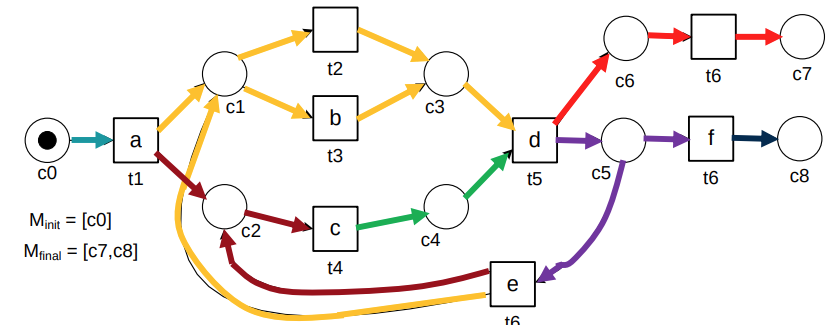
\includegraphics[width=0.8\textwidth]{maximal_decomposition.png}
    \caption{Maximal decomposition construction.}
    \label{fig:maximal_decomposition-png}
\end{figure}

\subsection*{Alignment Computation}

It is known that a trace fits the model $\iff$ it fits each of the fragments in a valid decomposition of this model.

Now to calculate the alignment costs, one must ponder the weights of the misalignments by the amount of times the misaligned activity appears in all of the fragments. Still, \emph{this will give a lower bound for the misalignment cost}.

\section*{Region-Based Mining}

Deals with the \textbf{synthesis problem}.

\begin{description}
    \item[State-based regions] can be used to construct a Petri net from a transition system.
    \item[Language-based regions] can be used to construct a Petri net from a prefix-closed language.
\end{description}

\subsection*{State-Based Regions}

Transition Systems are like low-level models, similar to state-machines, that "run" through the traces, interpreting activities as transitions.

\begin{figure}[h]
    \centering
    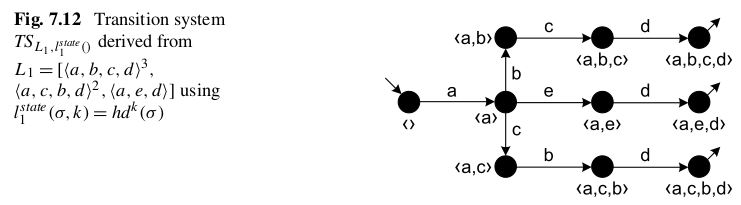
\includegraphics[width=0.8\textwidth]{transition-system.png}
    \caption{Transition System example}
    \label{fig:transition-system-png}
\end{figure}

Then we synthesize the TS into Petri Nets through regions.

\begin{definition}
    (State-based region) Given a transition system $TS=(S,A,T)$ over $S$ the set of states, $A$ the set of activities, and $T$ the transition rules, $R \subset S$ is a \emph{region} if, $\forall a\in A$, one of the following holds:
    \begin{itemize}
	\item All transitions $(s_1,a,s_2)\in T$ \emph{enter} $R$, \emph{i.e.}, $s_1\not\in R$ and $s_2\in R$; or
	\item All transitions $(s_1,a,s_2)\in T$ \emph{exit} R, \emph{i.e.}, $s_1\in R$ and $s_2\not\in R$; or
	\item All transitions $(s_1,a,s_2)\in T$ \emph{do not cross} R, \emph{i.e.}, $s_1,s_2\in R$ or $s_1,s_2\not\in R$.

    \end{itemize}
\end{definition}

Then, one maps the regions to places of a PN.

\subsection*{Language-Based Regions}

Based on the idea that a PN containing only transitions has the most modeling power (allows for any behavior), then, adding places restricts the behavior allowed.

In this scenario, a \emph{region} is defined by a set of input and a set of output transitions $X$ and $Y$ that are not affected by the insertion of a place $p_R$ connected to those ($\cdot p_R=X$, $p_R\cdot =Y$) containing at most 1 token. That is, this place does not disable the execution of any traces. This means that, when replaying any trace on the model with the addition of this new place, the number of tokens in $p_R$ must not be negative for any $k$-th event.

\begin{definition}
    (Language-based region) Given an event log $L\in \mathbb{B}(\mathcal{A}^{*})$, $R=(X,Y,c)$ is a \emph{region} of $L$ $\iff$:
    \begin{itemize}
	\item $X\subset \mathcal{A}$ is the set of input transitions of $R$;
	\item $Y\subset \mathcal{A}$ is the set of output transitions of $R$;
	\item $c\in {0,1}$ is the initial marking of $R$; and
	\item $\forall \sigma \in L$,$k\in {1,\ldots,|\sigma|}$,$\sigma_1=head^{k-1}(\sigma)$,$a=\sigma(k)$, $\sigma_2=head^{k}(\sigma)=\sigma_1 \oplus a$, it holds that \[
		c + \sum_{t\in X} \partial_{multiset}(\sigma_1)(t) - \sum_{t\in Y} \partial_{multiset}(\sigma_2)(t) \ge 0
	\] 
    \end{itemize}
\end{definition}

The first summation of the inequation represents the input tokens that are generated by that trace (so the amount of times each of the input transitions in $X$ was activated up until the $k$-th activity in the trace), while the second summation represents the consumed tokens (similar to the first, but for the output transitions in $Y$ and includes the $k$-th activity $a$).

\begin{note}
    Remember that a multiset can be seen as a function that takes one of its members and returns its amount.
\end{note}

Now if we understand $x_t\in {0,1}$ as the consumption of token, for transition $t$, of place $p_R$ ($x_t = 1$ if activity  $t$ consumes a token of $p_R$, $0$ otherwise), we can reformulate the equation in the definition as \[
    c + \sum_{t\in X\setminus tail^{k}(\sigma)}x_t - \sum_{t\in X\setminus tail^{k+1}(\sigma)}y_t \ge 0
\] for every non-empty prefix of the language/log (that is the meaning of $X\setminus tail^{k}(\sigma)$). So we get an inequation system whose solutions are possible $p_R$, \emph{i.e.}, \emph{possible regions}.

\begin{definition}
    (Language-based region) Given an event log $L\in \mathbb{B}(\mathcal{A}^{*})$, a triple $R=(x,y,c)$, with $x,y \in \left\{ 0,1 \right\}^{|\mathcal{A}|}$ and $c\in \left\{0,1\right\}$, is a \emph{region} of $L$ $\iff \forall w=w'\oplus a \in \overline{L}$, $w'\in L$ and $a\in \mathcal{A}$ \[
	c + \sum_{t\in \mathcal{A}}\left( w'(t)^{T}x(t) - w(t)^{T}y(t) \right) \ge 0
    \].
\end{definition}

In here, $w,w'$ are non-empty prefixes of the log ($\overline{L}$ is the prefix closure of $L$), which are regarded as multisets, therefore, $w'(t)$ returns the amount of times $t$ was executed before the $a$ event (same for $w$, but includes the event $a$).

One can also give an alternative definition.

\begin{definition}
    (Alternative Definition) Given an event log $L\in \mathbb{B}(\mathcal{A}^{*})$, a triple $R=(x,y,c)$, with $x,y \in \left\{ 0,1 \right\}^{|\mathcal{A}|}$ and $c\in \left\{0,1\right\}$, is a \emph{region} of $L$ $\iff$ \[
	c \bm{1} + A'x - Ay \ge \bm{0}
	\] where $A$ and $A'$ are defined as $A(w,t) = w(t)$ and $A'(w,t)=w'(t)$, with  $w=w'\oplus a \in \overline{L}$, $w'\in L$ and $a\in \mathcal{A}$.
\end{definition}

\subsubsection*{Finding Workflow Nets}

Still, the solutions of the inequation do not provide a workflow net, as there can be multiple overlapping states.

\begin{definition}
    (Minimal Region) Given a log  $L$ and a region $R=(x,y,c)$, we say that $r$ is \emph{minimal} if there do not exist two other, non-trivial regions $r_1,r_2$ with $r_1=(x_1,y_1,c_1)$ and $r_2=(x_2,y_2,c_2)$ such that $x = x_1+x_2$ and $y=y_1+y_2$ and $c=c_1+c_2$.
\end{definition}

Yet, this does not guarantee a region/place is not redundant. Redundancy is when a place has the same marking a set o places that does not include the original.

To find a feasible WF net, one can understand this as a Integer Linear Programming problem. The following formulation guarantees to find not only feasible regions, but also minimal regions.

\begin{definition}
    (ILP formulation) Given a log $L$ and $A, A'$ as in the previous definition. The \emph{ILP} is defined as:
    \begin{equation}
        \begin{aligned}
	    \min_{x,y} \quad & c + \bm{1}^{T}\left( c \bm{1} + A(x-y) \right) \\
	    \text{s.t.} \quad & c \bm{1} + A'x - Ay \ge \bm{0} \\
			     & \bm{1}^{T}x + \bm{1}^{T}y \ge 0 \\
			     & \bm{0} \le x\le \bm{1} \\
			     & \bm{0} \le y\le \bm{1} \\
			     & 0 \le c\le 1
        \end{aligned}
    \end{equation}
\end{definition}

As far as I understood, the loss function counts the amount of remaining tokens from the prefix closure of the log. In $\bm{1}^{T}A(x-y)$, each row of the matrix multiplication $A(x-y)$ is the sum of tokens added to and removed from the place, so by multiplying this to the left by $\bm{1}^{T}$, we just sum these values, that we already know are all $\ge 0$.

This formulation, however, does not guarantee that a WF-net is achieved, as it provides a single solution. So we add further constraints.

The first set of constraints is to use the causal dependencies derived from the log. That is, for each causal dependency, one can extend the former ILP formulation with the constraint that the place must fulfil the causal relation.

\begin{definition}
    (ILP for causal dependency) Given a log $L$ and $A, A'$ as in the previous definition. Furthermore, given two transitions $t_1,t_2\in \mathcal{A}$ and assuming $t_1\to t_2$, we extend the ILP formulation with two extra bounds, namely: \[
	x(t_1)=y(t_2)=1
    \].
\end{definition}

Therefore, solving the above-defined ILP for each causal dependency derived from the log, one can construct a PN able to replay the log.

\begin{description}
    \item[Workflow net:] to guarantee that the resulting PN has source and sink places, one must add a $c=0$ constraint when searching for places for causal dependencies and separately search for the source place ($c=1 \land \bm{1}^{T}x=0$) and the sink place ($c=0 \land \bm{1}^{T}y=0$).
    \item[Empty after completion:] to guarantee that there will be no tokens left after playing a trace, one must add $c+\sigma^{T}x - \sigma^{T}y=0$ constraints for every $\sigma \in L$ to all ILP problems.
\end{description}

\section*{TL;DR}

\begin{description}
    \item[Fitness] is the capacity of a model to allow for the behavior seen in the log.
    \item[Simplicity] is defined by the Occam's Razor, \emph{i.e.}, the least amount of complexity necessary.
    \item[Precision] is the characteristic of a model that does not allow for unseen behavior, \emph{i.e.}, that is not underfitting.
    \item[Generalization] is when a model does not overfits the data, \emph{i.e.}, it does not restricts itself to behavior to the examples seen in the log.
\end{description}

\begin{definition}
    (Escaping edges) We define the \emph{escaping edges precision} through \[
    ee_p(A_A) = \frac{1}{\sum_{s \in Q} \omega(s)}\sum_{s \in Q} \omega(s) \frac{e_x(s)}{a_v(s)}
    \] 
\end{definition}

\begin{note}
    \textbf{Watch out!} Neither the starting state ($\epsilon$) nor the ending states are counted in the \emph{escaping edges} precision metric.
\end{note}

\begin{description}
\item[alignment alternative] \[
	fitness(L,N) = 1 - \frac{f_{cost}(L,N)}{move_L(L) + \|L\|\cdot move_N(N)}
    \] where 
    \begin{itemize}
        \item $f_{cost}$ is the sum of alignment costs of all traces in the log (\textbf{watch out for repeated traces});
	\item $move_L$ are the log moves performed, which is equal to the number of events (\textbf{again, watch out for repeated traces});
	\item $\|L\|$ is the amount of traces in the log;
	\item $move_N$ is the number of model moves, that is, the length of the smallest trace allowed by the model.
    \end{itemize}
\end{description}

\begin{definition}
    (Marking equation) Given $s,s'$ markings in the vector form, then, \textbf{if $s'$ is reachable from $s$ $\iff$ $\exists \varrho\in \N^{|A|}$ such that the marking equation \[
	s + N\cdot \varrho = s'
\] holds.}
    Above, $N$ is the \emph{incidence matrix}, defined as \[
	N(p_i, t_j) = 
	\begin{cases}
	    -1 & \text{if } p_i \in \cdot t_j \\
	    1 & \text{if } p_i \in t_j\cdot  \\
	    0 & \text{otherwise}
	\end{cases}
    \], it maps the consumption and production of tokens by the activities.
\end{definition}

\begin{note}
    One can decompose the net by generating sub-nets for each place, splitting at every transition. Then, if there are invisible transitions, one must continue the sub-net through them. Lastly, merge all the subnets that contain transitions that are not unique. A maximal valid decomposition is achieved.
\end{note}

\begin{figure}[h]
    \centering
    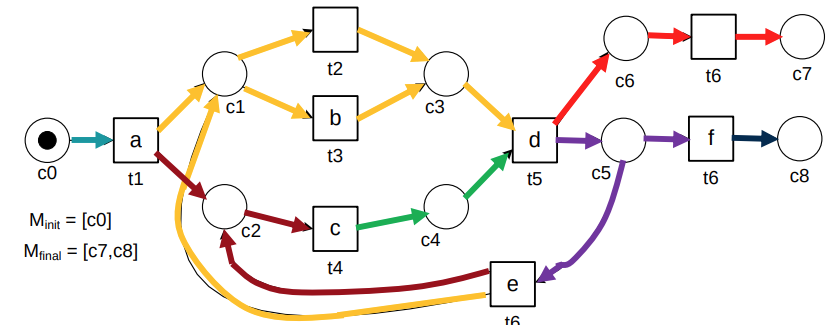
\includegraphics[width=0.8\textwidth]{maximal_decomposition.png}
    \caption{Maximal decomposition construction.}
    \label{fig:maximal_decomposition-png}
\end{figure}

\begin{definition}
    (Alternative Definition) Given an event log $L\in \mathbb{B}(\mathcal{A}^{*})$, a triple $R=(x,y,c)$, with $x,y \in \left\{ 0,1 \right\}^{|\mathcal{A}|}$ and $c\in \left\{0,1\right\}$, is a \emph{region} of $L$ $\iff$ \[
	c \bm{1} + A'x - Ay \ge \bm{0}
	\] where $A$ and $A'$ are defined as $A(w,t) = w(t)$ and $A'(w,t)=w'(t)$, with  $w=w'\oplus a \in \overline{L}$, $w'\in \overline{L}$ and $a\in \mathcal{A}$.
\end{definition}

In here, $w,w'$ are non-empty prefixes of the log ($\overline{L}$ is the prefix closure of $L$), which are regarded as multisets, therefore, $w'(t)$ returns the amount of times $t$ was executed before the $a$ event (same for $w$, but includes the event $a$).

\begin{definition}
    (ILP formulation) Given a log $L$ and $A, A'$ as in the previous definition. The \emph{ILP} is defined as:
    \begin{equation}
        \begin{aligned}
	    \min_{x,y} \quad & c + \bm{1}^{T}\left( c \bm{1} + A(x-y) \right) \\
	    \text{s.t.} \quad & c \bm{1} + A'x - Ay \ge \bm{0} \\
			     & \bm{1}^{T}x + \bm{1}^{T}y \ge 0 \\
			     & \bm{0} \le x\le \bm{1} \\
			     & \bm{0} \le y\le \bm{1} \\
			     & 0 \le c\le 1
        \end{aligned}
    \end{equation}
\end{definition}

As far as I understood, the loss function counts the amount of remaining tokens from the prefix closure of the log. In $\bm{1}^{T}A(x-y)$, each row of the matrix multiplication $A(x-y)$ is the sum of tokens added to and removed from the place, so by multiplying this to the left by $\bm{1}^{T}$, we just sum these values, that we already know are all $\ge 0$.

\begin{definition}
    (ILP for causal dependency) Given a log $L$ and $A, A'$ as in the previous definition. Furthermore, given two transitions $t_1,t_2\in \mathcal{A}$ and assuming $t_1\to t_2$, we extend the ILP formulation with two extra bounds, namely: \[
	x(t_1)=y(t_2)=1
    \].
\end{definition}

Therefore, solving the above-defined ILP for each causal dependency derived from the log, one can construct a PN able to replay the log.

\begin{description}
    \item[Workflow net:] to guarantee that the resulting PN has source and sink places, one must add a $c=0$ constraint when searching for places for causal dependencies and separately search for the source place ($c=1 \land \bm{1}^{T}x=0$) and the sink place ($c=0 \land \bm{1}^{T}y=0$).
    \item[Empty after completion:] to guarantee that there will be no tokens left after playing a trace, one must add $c+\sigma^{T}x - \sigma^{T}y=0$ constraints for every $\sigma \in L$ to all ILP problems.
\end{description}

\end{document}
